In this section, we present a tool for extracting~\emph{scenarios} from
blocks of instructions.~\todo{include scenario definition from Alessandro's journal paper
together with a reference.}

To mine scenarios from blocks of instructions, we partially reuse the methodology
used for construction of the concurrency oracles from the previous section. The methodology
involves calculating the set of static dependencies of the block of instructions,
constructing the~\emph{unfolded} static dependencies graph~\footnote{Similar to one in the
figure~\ref{fig-example-graph}, but with with data-vertexes duplicated on every update.};
and then wiping out the data-vertexes preserving the transitive connections
of instruction-vertexes. A~\emph{transitive closure} of the resulting graph will
display the partial order on the set of events represented as instruction-vertexes.
\todo{Make this a good-looking algorithm}.

Extraction of scenarios from programs enables us to use the associated methods for
compiling programs into application-specific hardware. The Conditional Partial
Order Graphs formalism enables synthesis of scenarios, allowing to compile them into
a circuit with some functionality shared.

\begin{figure}
\vspace{-4mm}
\centerline{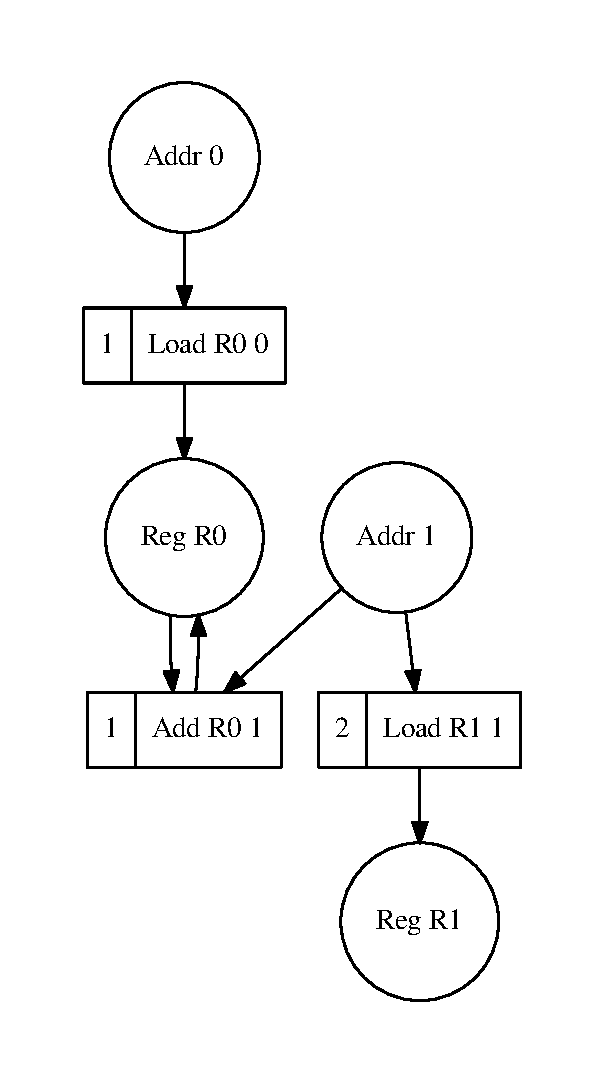
\includegraphics[scale=0.6]{img/oracle2.pdf}}
\vspace{-3mm}
\caption{An overlay of static dependency graphs of two blocks of instructions.\label{fig-example-graph}}
\vspace{-9mm}
\end{figure}